Edge computing \cite{Edge} is an open platform that integrates network, computing, storage, and application core
capabilities on the edge of the network that is physically close to the data source. It provides
a computing model for edge intelligence services. The location where the edge calculation occurs is 
called the edge node, which can be any node between the data generation source and the cloud center
that has computing resources and network resources. The amount of devices connected to the 
internet, and as a consequence the amount of data shared, is constantly growing and this introduced 
a number of different problems that have to be addressed. 
\\
\begin{enumerate}
    \item First of all the high amount of traffic flowing in the network is making bandwidth a
            bottleneck for the traditional cloud computing approach. 

    \item With the popularity of smart home, video data for many families in the house installation
            network camera, privacy and data security will be a problem since data will be collected
            and directly uploaded to the cloud computing increasing the risk of disclosure of users 
            personal data.

    \item As more and more user applications run on cloud servers, the demand for energy consumption
            in large-scale data centers will be difficult to meet in the future. The existing research on
            energy consumption in cloud computing centers focuses on how to improve energy efficiency.
            However,improving energy efficiency alone will not solve the enormous energy consumption 
            problem of the data center, which will be more prominent in the environment of all things.
\end{enumerate}

In response to this, the development of the application requirements of the Internet of Everything has 
spawned an edge computing model. The edge computing model is a new type of computing model that performs
calculations at the edge of the network. In the edge computing model, the edge device has the processing
capability of performing calculation and data analysis, and migrates some or all of the computing tasks
performed by the original cloud computing model to the network edge device, reducing the computing load
of the cloud server, slowing down the pressure of the network bandwidth, and improving the processing 
efficiency of data in the era of Internet of Everything. Edge computing is not to replace the cloud, 
but to complement the cloud, providing a better computing platform for related technologies such as mobile
computing and the Internet of Things.

Existing research generally divides the architecture of edge computing from the central network to the 
edge of the network into three layers: the cloud computing layer, the edge computing layer, and the ending
layer, as shown in Figure \ref{fig:edge_infr}. Different layers are generally divided according to their computing 
and storage capabilities. The computing and storage capabilities of the ending layer, the edge computing
layer, and the cloud computing layer are sequentially increased. In order to achieve intra-layer and
cross-layer communication, each communication technology can be connected by various communication 
technologies, including wired communication (such as Ethernet, optical fiber), wireless communication 
(such as Bluetooth, LTE, ZigBee, NFC, IEEE802.11a/b). /c/g/c, satellite link) or a combination of two 
technologies. Edge computing extends cloud services to the edge of the network by introducing an edge 
layer between the terminal device and the cloud.

\begin{figure}
    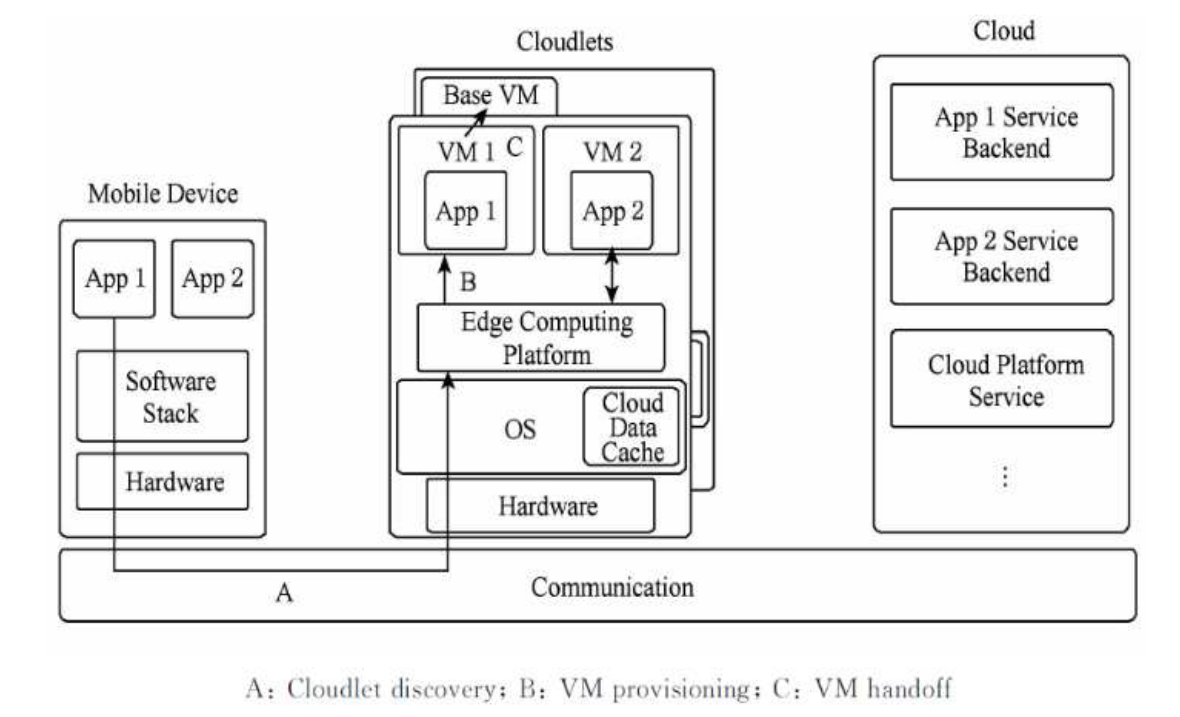
\includegraphics[width=\textwidth]{Images/Edge_infrastructure.png}
    \caption{Edge computing infrastructure.}
    \label{fig:edge_infr}
\end{figure}
